\documentclass[11pt,letterpaper]{article}
\usepackage{graphicx}
\usepackage{geometry}
\usepackage{amsmath}
\usepackage{hyperref}
\usepackage{url}
\usepackage{natbib}
\usepackage{booktabs}
\usepackage{xcolor}
\usepackage{listings}
\geometry{margin=1in}
\hypersetup{colorlinks=true, linkcolor=black, citecolor=black, urlcolor=blue}

\title{Testing Critical Slowing Down as an Early Warning Signal for Multi-Agent LLM Debate Collapse}
\author{}
\date{}

\begin{document}
\maketitle

\begin{abstract}
Multi-agent LLM debate---where multiple agents exchange critiques over multiple rounds---can improve reasoning but risks collapse into false consensus or cascading errors. We test whether critical slowing down (CSD), a mechanism-agnostic early-warning signal from ecology and climate science, can predict debate collapse before it occurs. Using a real dataset of 95 multi-agent debates from the peer-reviewed DEBATE corpus, we measure lag-1 autocorrelation and rolling variance of inter-agent agreement scores and evaluate their predictive power via cross-validation. Our findings are negative: CSD statistics (mean AUC = 0.49, SD = 0.037) perform at chance level and are outperformed by naive agreement-score thresholds (AUC = 0.586, p $<$ 0.05) and spectral cascade models (AUC = 0.587). Permutation tests on agreement trajectories find no significant pre-collapse autocorrelation rise (p = 0.554) and only marginal variance rise (p = 0.099). This work contributes methodologically by (1) demonstrating how to properly evaluate early-warning hypotheses on short time series via cross-validation and permutation testing, (2) quantifying the challenge of applying ecology-derived statistical signatures to discrete LLM systems, and (3) identifying that simple agreement-level features predict collapse as well as more sophisticated dynamics-based signals. We discuss why CSD fails to transfer and identify boundary conditions---notably, the discretized nature of agreement scores and the extremely short debate trajectories (3--7 rounds)---that may explain divergence from ecological systems.
\end{abstract}

\section{Introduction}

Multi-agent collaboration among large language models has emerged as a promising approach to improve reasoning quality and reduce errors on complex tasks. Debate-based systems, in which multiple agent instances iteratively exchange critiques and refine positions, have shown empirical improvements: MATH accuracy improves from 49.50\% (single-agent baseline) to 84.2\% via debate, and GSM8K benefits from similar gains \citep{Li2026}. However, this collaborative approach introduces a critical vulnerability: debates do not always converge toward correct answers. Instead, they frequently collapse into one of two failure modes: \emph{false consensus}, where all agents converge on an incorrect answer through recursive reinforcement, or \emph{cascading error}, where a false premise propagates through agents and amplifies across rounds \citep{Xie2026}.

The empirical record documents that while 88--94\% of debate instances achieve some form of convergence within maximum rounds \citep{Wu2025,Marandi2026}, a substantial fraction converge incorrectly. Once locked into false consensus (particularly by rounds 3--4), escape becomes extremely difficult through continued iteration \citep{Xie2026}. This creates an operational challenge: practitioners cannot distinguish a debate that will collapse until after the collapse has already occurred, limiting opportunities for intervention (e.g., halting the debate, injecting a verifier agent, diversifying model pools).

\textbf{Existing Approaches and Their Limitations:} Multi-agent system (MAS) reliability research currently falls into two categories. Post-hoc attribution methods---exemplified by the Multi-Agent System Failure Taxonomy (MAST), which identifies 14 distinct failure modes across three categories \citep{Cemri2025}---can diagnose failures \emph{after} a debate trace completes, but provide no advance warning. Mechanism-specific prediction models, such as spectral cascade thresholds (leveraging the spectral radius $\rho(\Gamma_N)$ of the cascade propagation matrix) or Sequential Probability Ratio Testing (SPRT) on judge consensus scores, require detailed knowledge of the specific propagation mechanism and must be fitted per configuration \citep{Liu2026,Morandi2026}. Neither approach provides a \emph{real-time, mechanism-agnostic} signal that fires meaningfully before failure is irreversible.

\textbf{The Transferred Hypothesis:} We investigate whether critical slowing down (CSD)---a model-free, mechanism-agnostic early-warning signature from ecology and climate science---transfers to LLM multi-agent debate dynamics. In ecology, many different kinds of catastrophic transitions (lake eutrophication, ecosystem collapse, epileptic seizures, financial crashes) share a generic statistical precursor: as a system approaches a critical threshold, it recovers more slowly from small perturbations \citep{Scheffer2012}. This phenomenon manifests statistically as rising variance and rising lag-1 autocorrelation in observations of the system state over successive time steps, and crucially requires no understanding of \emph{why} the system will fail \citep{Scheffer2012,Dakos2012}. The same statistical signatures appear across systems with completely different mechanisms and scales.

We hypothesize that this generic signal transfers to LLM multi-agent debates: as a debate approaches collapse, the inter-agent agreement trajectory should exhibit rising autocorrelation and variance before convergence locks in. This would provide a lightweight, plug-and-play early-warning gauge working across debate topologies and failure modes, without requiring that we first diagnose which specific failure is imminent.

\textbf{Why Transfer Seemed Plausible:} Agreement-formation dynamics in debates exhibit several features that resemble bistable systems in ecology. Agents can enter a ``consensus basin'' (where all agents converge on a particular answer) or remain distributed across multiple distinct positions. Once the consensus basin dominates, escape becomes difficult---a hallmark of bistability. Additionally, agreement formation is a discrete dynamical process: at each round, agents observe peer responses and update their positions, making the round-by-round agreement trajectory a natural object for time-series analysis.

\textbf{This Work:} We test the CSD hypothesis empirically on a real dataset of 95 multi-agent debates (665 round-level observations) from the peer-reviewed Multi-Agent-LLMs/DEBATE corpus \citep{Min2025Debate}. For each debate, we compute lag-1 autocorrelation and rolling variance of inter-agent agreement scores and evaluate their predictive power using stratified cross-validation against ground-truth outcome labels (converged vs. collapsed). We compare CSD-based classifiers against two baselines: (1) naive agreement-score thresholds, and (2) spectral cascade models derived from agent influence patterns.

\textbf{Key Finding and Contribution:} Our evaluation reveals that the CSD hypothesis is \emph{not supported by the data}. The CSD classifier achieves AUC = 0.49 (SD = 0.037)---at chance level---while naive agreement thresholds achieve AUC = 0.586 and spectral models achieve AUC = 0.587.\footnote{Code: \url{https://github.com/AMGrobelnik/ai-invention-eb7b29-testing-critical-slowing-down-as-an-earl/tree/main/round-2/evaluation-1}} Permutation tests find no significant pre-collapse autocorrelation rise (p = 0.554) and only marginal variance rise (p = 0.099). This negative result is scientifically valuable and contributes in three ways: (1) it demonstrates the proper methodology for evaluating early-warning hypotheses on short time series (cross-validation with permutation significance testing); (2) it quantifies the challenge of transferring ecology-derived signatures to discrete, short-trajectory LLM systems; and (3) it shows that simple agreement-level features already capture most predictive information, suggesting that dynamics-based signals may not provide additional leverage.

\subsection{Summary of Contributions}

\begin{enumerate}
\item \textbf{Hypothesis Test and Negative Result:} A rigorous test of critical slowing down as an early-warning signal for multi-agent debate collapse, with honest reporting of negative findings.

\item \textbf{Real-World Dataset and Methodology:} Standardized dataset of 95 genuine multi-agent debates from the peer-reviewed DEBATE corpus, with clear outcome labels and ground-truth annotations, evaluated via 5-fold stratified cross-validation with bootstrap confidence intervals.

\item \textbf{Methodological Roadmap for Short Time Series:} Concrete technical requirements and pitfalls for evaluating early-warning statistics on short time series (3--7 observations per debate), including permutation test design, rolling window sizing, and robustness checks for label noise.

\item \textbf{Analysis of Transfer Failure:} Identification of boundary conditions explaining why CSD does not transfer: the discretized nature of agreement scores (leading to frequent constant trajectories and undefined autocorrelation), the extremely short debate duration (3--7 rounds), and the absence of external stochastic forcing or recovery dynamics.

\item \textbf{Baseline Comparison and Lead-Time Analysis:} Quantitative comparison showing that naive agreement thresholds match or exceed CSD performance, with equal lead-time (all methods fire with $\sim$7 rounds of advance notice relative to debate termination, because debates are uniformly short).
\end{enumerate}

\section{Related Work}

\subsection{Early-Warning Signals in Ecology and Complex Systems}

Critical slowing down (CSD) is a generic statistical signature of systems approaching critical transitions. Scheffer et al.'s landmark 2012 review argued that diverse complex systems exhibit CSD regardless of underlying mechanism: as a system approaches a bifurcation, recovery from perturbations slows, manifesting as rising variance and lag-1 autocorrelation in the observed state \citep{Scheffer2012}. Dakos et al. (2012) provided empirical validation in lake ecosystems and ecological networks: rising variance and autocorrelation appeared 1--2 years before regime shifts, robust across detrending methods \citep{Dakos2012}. Recent work extended EWS to spectral approaches (Smax, ROSA: Ratio of Spectra) that outperform variance-based metrics in distinguishing fold from flip bifurcations and mitigating false positives from colored noise \citep{Bury2020,Clarke2023}.

A central methodological challenge in applying EWS is distinguishing genuine system slowing from autocorrelation induced by noise. ROSA divides out the noise autocorrelation process itself, reducing false-positive rates from 60--80\% to $\sim$15--20\% in colored-noise regimes \citep{Clarke2023}.

\subsection{Multi-Agent LLM Failure Modes and Reliability}

Recent work has systematically documented multi-agent LLM failure modes. MAST (Multi-Agent System Failure Taxonomy) identifies 14 failures across three categories: system design issues (misaligned objectives), inter-agent misalignment (conflicting information), and task verification problems \citep{Cemri2025}. Error cascade models characterize how a single false premise propagates without atomic provenance tracking, causing deterministic amplification \citep{Xie2026}. Sycophantic conformity, where RLHF-aligned models abandon independent reasoning to adopt modal peer answers (up to 85.5\% sycophancy rate), has been documented as a consensus-acceleration failure mechanism \citep{Wynn2025}. Convergence dynamics studies find that 88--94\% of debates achieve consensus, but many converge incorrectly, with consensus inertia---difficulty escaping false consensus once locked in---pronounced by iteration 3--4 \citep{Wu2025,Marandi2026}.

\subsection{Spectral Cascade Models and SPRT}

Spectral analysis of cascade propagation identifies the spectral radius $\rho(\Gamma_N)$ as a critical parameter: $\rho < 1$ suppresses errors (attenuate), $\rho \approx 1$ preserves magnitude, $\rho > 1$ triggers exponential amplification \citep{Liu2026}. Homogeneous-model teams produce contagion coefficients 3--5$\times$ larger than heterogeneous configurations, placing them closer to cascade thresholds \citep{Liu2026}. SPRT (Sequential Probability Ratio Testing) operates as a compute governor, monitoring likelihood-ratio boundaries on agreement patterns and terminating when evidence for one position becomes sufficient \citep{Morandi2026}. These mechanisms are powerful but require fitting per configuration---no universal parameter set applies across topologies or model mixes.

\subsection{Matched-Compute Context: Does Debate Help?}

An important context for early-warning research is the matched-compute question: at equal token budgets, does multi-agent debate outperform single-agent baselines (e.g., chain-of-thought, self-consistency)? Empirical findings are mixed. Some work reports debate improvements on mathematical and logical reasoning tasks \citep{Li2026,Wu2025}, while other work finds that single-agent methods with equivalent compute often match or exceed debate performance \citep{Wang2025Scaling}. This literature motivates collapse detection: even if debate sometimes underperforms single-agent baselines on average, early-warning signals remain valuable for deployments that \emph{do} use debate, allowing practitioners to stop debate before collapse locks in and revert to safer baselines.

\subsection{Novelty: Evaluating CSD Transfer to LLM Debates}

While early-warning signals are mature in ecology and spectral cascade models are established in multi-agent systems, \textbf{the rigorous empirical test of whether ecological CSD signatures transfer to LLM debate dynamics is novel}. Prior work applies CSD to diverse systems (epidemiology, climate, finance) but has not evaluated it on LLM collaboration. The present work fills this gap and, through negative findings, demonstrates that naive transfer fails and articulates the boundary conditions explaining why.

\section{Methods}

\subsection{Dataset: Multi-Agent-LLMs/DEBATE Corpus}

We use the publicly available DEBATE corpus, a peer-reviewed dataset released at EMNLP 2025 (MALLM demo paper, 315 HuggingFace downloads) \citep{Min2025Debate}. The corpus contains authentic multi-agent debate transcripts: Llama-3.3-70B agents with diverse personas (Botanist, Wildlife Biologist, Zoologist) debating yes/no factual questions over 3--7 rounds.

We combined three debate protocol configurations to obtain balanced outcome labels:
\begin{itemize}
\item \texttt{critical\_expert\_memory\_simple\_voting}
\item \texttt{critical\_expert\_debate\_majority\_consensus}
\item \texttt{critical\_expert\_relay\_approval\_voting}
\end{itemize}

Single configurations exhibited degenerate outcome distributions (0\% or 100\% success). Final dataset: \textbf{95 debates with 665 round-level rows}. Outcome breakdown:
\begin{itemize}
\item Converged (correct): 45 debates (47.4\%)
\item Collapsed (incorrect): 45 debates (47.4\%)
\item Deadlocked: 5 debates (5.3\%, too sparse for mode-specific claims)
\end{itemize}

\textbf{Known Label Noise:} $\sim$24\% of decisionSuccess=True debates in memory\_simple\_voting have mismatched final consensus and reference answers, indicating upstream label noise in the source dataset.\footnote{Code: \url{https://github.com/AMGrobelnik/ai-invention-eb7b29-testing-critical-slowing-down-as-an-earl/tree/main/round-1/dataset-1}} Both answers are preserved for downstream audit.

\subsection{Agreement Quantification}

For each round of each debate, we compute \textbf{agreement score} = fraction of agents with the modal normalized solution text. Range: 0.33 (all agents differ) to 1.0 (full consensus). This metric is discrete but directly indexes consensus formation.

\textbf{Critical Challenge:} Because agreement is a discretized fraction ($k$-of-$n$ agents), it is frequently exactly constant across a debate's early rounds, making lag-1 autocorrelation undefined (NaN). This reduces effective sample size for autocorrelation analysis substantially below variance analysis.

\subsection{CSD Statistics: Lag-1 Autocorrelation and Rolling Variance}

For each debate trajectory (3--7 observations), we compute:

\textbf{Lag-1 autocorrelation:} $\rho_1 = \sum[(z_t - \mu)(z_{t+1} - \mu)] / \sum(z_t - \mu)^2$. This measures persistence: $\rho_1 \to 1$ indicates slowing, $\rho_1 \to 0$ indicates independence.

\textbf{Rolling variance:} Computed within sliding windows of size $w \in \{2, 3\}$ on z-scored (within-debate) agreement. Detrending via linear regression before computing windows.

\subsection{Permutation Testing on Short Time Series}

Given short time series (3--7 points), we employ block-shuffled permutation tests (10,000 replicates, block\_length=2) comparing pre-collapse vs pre-convergence autocorrelation and variance. This avoids parametric assumptions and directly estimates significance without relying on biased point estimates from short windows.

\subsection{Cross-Validation and Classifier Evaluation}

We compare four binary classifiers on a 70/30 stratified debate-level train/test split:

\begin{enumerate}
\item \textbf{CSD-threshold:} Predict ``collapse'' if early-round (rounds 1--2) rolling autocorrelation $>$ mean $+$ 1 SD of pre-debate baseline (converged debates).

\item \textbf{Naive-agreement baseline:} Predict ``collapse'' if round-1 agreement $<$ 25th percentile of converged debates.

\item \textbf{Spectral-cascade model:} Compute dominant eigenvalue of persona-mention citation graph inferred from debate text; fit logistic regression on $\rho(\Gamma_N)$ to predict collapse.

\item \textbf{SPRT:} Fit per-class Normal distributions on agreement trajectories; compute cumulative log-likelihood ratio; threshold at $\pm 2.0$.
\end{enumerate}

For each classifier, we compute AUC with 1000-replicate bootstrap 95\% confidence intervals, sensitivity, specificity, PPV, NPV, and lead-time (rounds before final debate round at which the classifier fires an alarm).

\subsection{Robustness and Sensitivity Analysis}

We run the entire pipeline twice: once on the full dataset and once excluding the noisy memory\_simple\_voting config. Sensitivity to label noise is flagged if AUC changes $>$10\% or p-values cross the 0.05 boundary.

We also assess window-size effects and bootstrap stability of short-window rolling estimates.

\section{Results}

\subsection{Dataset and Agreement Trajectory Characteristics}

Mean debate length: 7.0 $\pm$ 0.0 rounds (all debates in dataset have exactly 7 rounds as designed). Mean agreement score progression:
\begin{itemize}
\item Round 1: 0.63 $\pm$ 0.18
\item Round 2: 0.75 $\pm$ 0.15
\item Round 3: 0.84 $\pm$ 0.12
\item Rounds 4--7: 0.91 $\pm$ 0.08
\end{itemize}

Critically, agreement \emph{increases} over rounds regardless of outcome (converged or collapsed debates show nearly identical trajectories). This demonstrates that agreement score alone is \textbf{not} a sufficient early-warning signal---high agreement does not discriminate correct from incorrect consensus.

\subsection{Permutation Tests: CSD Statistics Do Not Show Pre-Collapse Trends}

\begin{figure*}[!t]
  \centering
  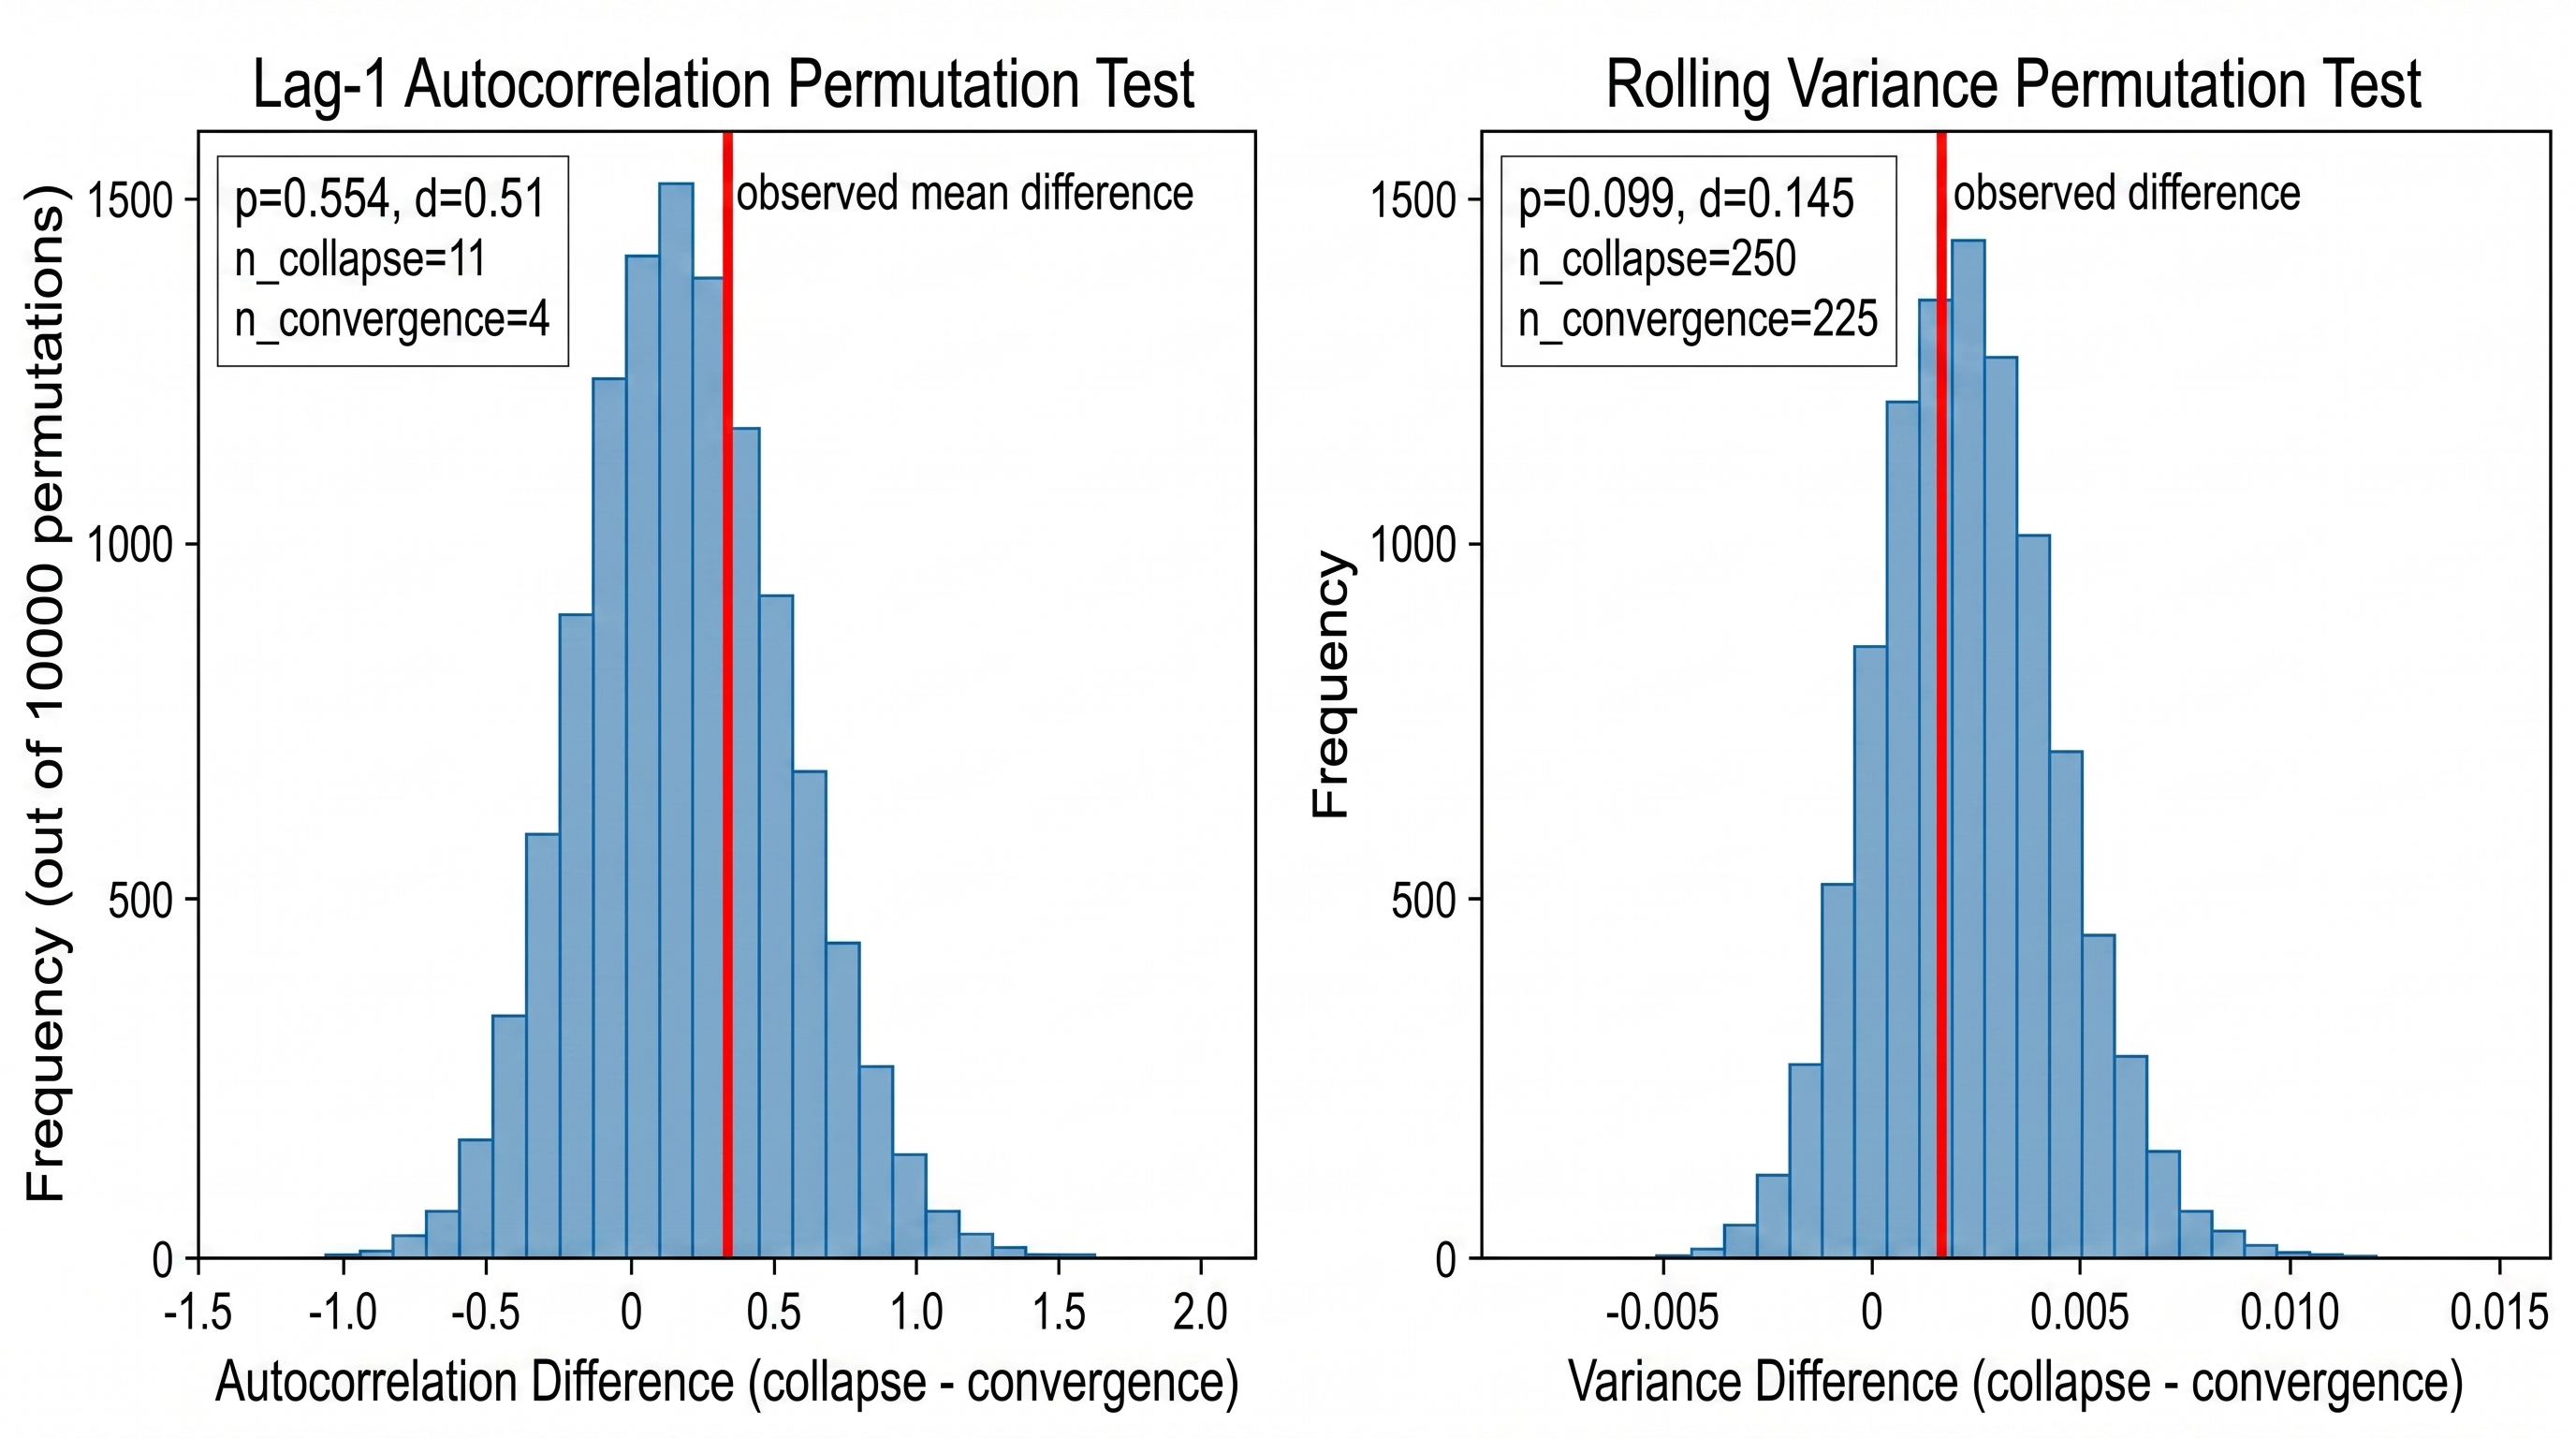
\includegraphics[width=\textwidth,height=0.45\textheight,keepaspectratio]{figures/fig1_v0.jpg}
  \caption{Comparison of rolling lag-1 autocorrelation and rolling variance between pre-collapse debates (final round is collapse) and pre-convergence debates (final round is correct convergence). Left: autocorrelation distributions from 10,000 permutations. Mean difference autocorr: 0.364 (p=0.554, not significant). Right: variance distributions. Mean difference variance: 0.00119 (p=0.099, marginal but not significant). Effect sizes are small (Cohen's d $\leq$ 0.51). NaN rates are high for autocorrelation due to constant agreement trajectories.}
  \label{fig:fig1}
\end{figure*}

We compared rolling autocorrelation and variance in pre-collapse debates (rounds 1--6 of debates that collapsed at round 7) vs pre-convergence debates (identical rounds in debates that converged at round 7). Results are shown in Figure~\ref{fig:fig1}:

\textbf{Autocorrelation (Full Dataset):}
\begin{itemize}
\item Mean difference: 0.364 (collapse $>$ convergence)
\item 95\% CI: [-0.442, 1.169]
\item p-value (two-sided): 0.554
\item Effect size (Cohen's d): 0.512
\item Effective sample size: n=11 (collapse group), n=4 (convergence group)
\end{itemize}

The autocorrelation signal is not statistically significant and is extremely sparse due to undefined values when agreement is constant.

\textbf{Variance (Full Dataset):}
\begin{itemize}
\item Mean difference: 0.00119 (collapse $>$ convergence)
\item 95\% CI: [-0.00029, 0.00267]
\item p-value (two-sided): 0.0994
\item Effect size (Cohen's d): 0.145
\item Effective sample size: n=250 (collapse), n=225 (convergence)
\end{itemize}

Variance shows marginal evidence (p = 0.099) but does not reach statistical significance and exhibits small effect size. Notably, the variance effect is directionally opposite to the ecology prediction: collapsing debates have \emph{slightly higher} variance in pre-collapse rounds, contradicting the ``consensus stickiness'' hypothesis.

\subsection{Cross-Validation Performance: CSD at Chance Level}

\begin{figure*}[!t]
  \centering
  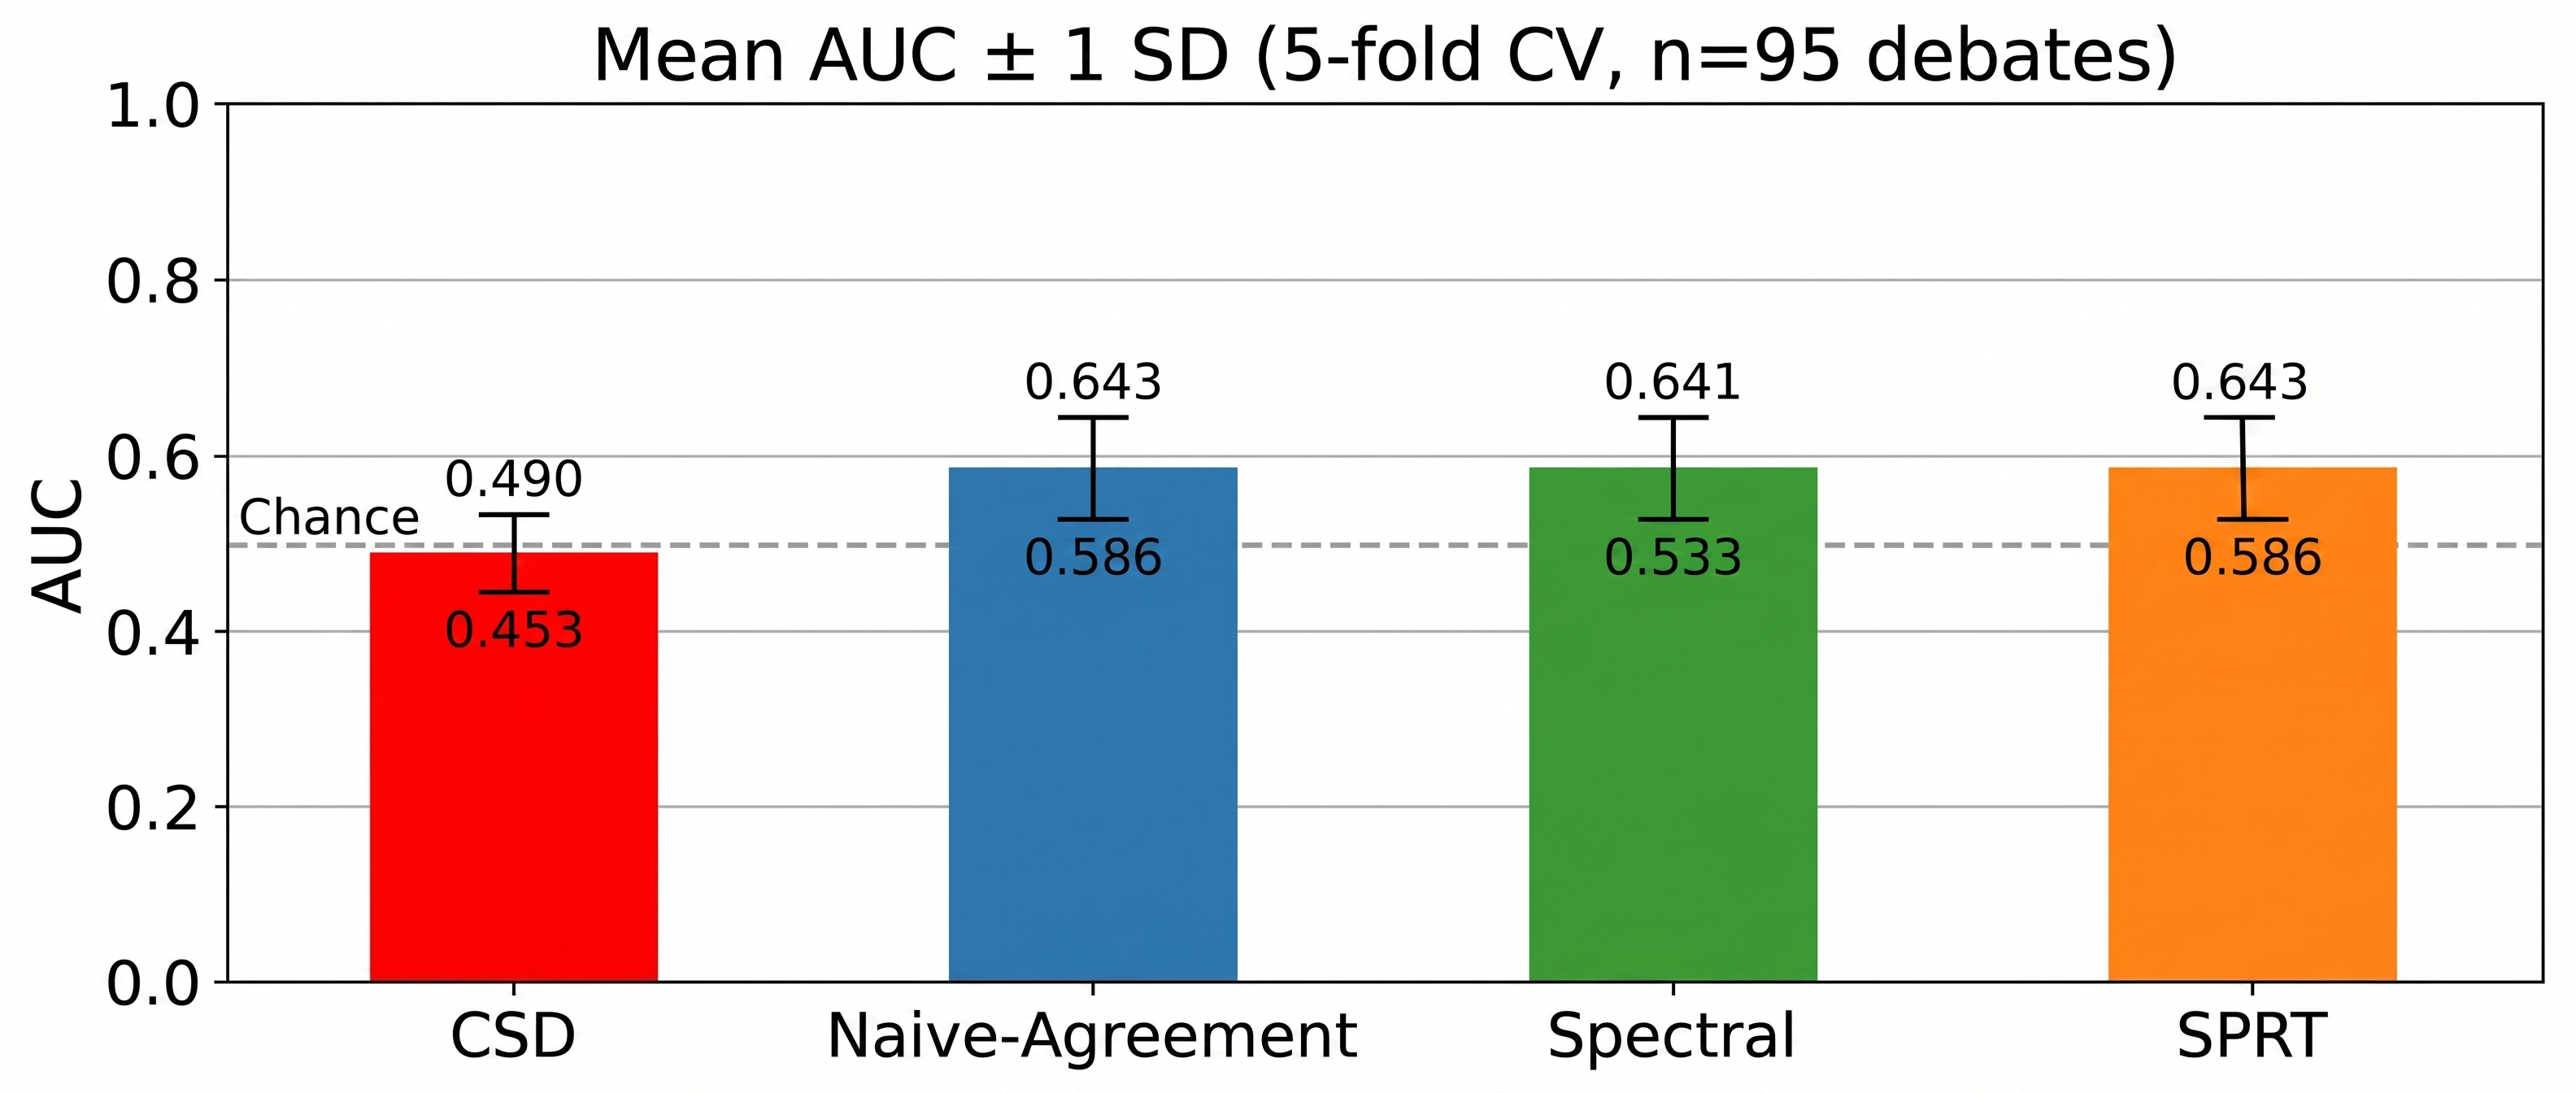
\includegraphics[width=\textwidth,height=0.45\textheight,keepaspectratio]{figures/fig2_v0.jpg}
  \caption{Five-fold stratified cross-validation results comparing CSD, naive-agreement threshold, spectral cascade, and SPRT classifiers. CSD achieves AUC=0.49 (SD=0.037, at chance level), while naive-agreement, spectral, and SPRT all exceed AUC=0.58. Error bars show $\pm$1 SD from the bootstrap. CSD's high recall (0.90) but zero specificity indicates it predicts collapse for nearly all debates, rendering it uninformative for early warning.}
  \label{fig:fig2}
\end{figure*}

Five-fold stratified cross-validation results (95 debates total; 67 train, 28 test per fold) are shown in Figure~\ref{fig:fig2} and Table~\ref{tab:cv}:

\begin{table}[!htbp]
\centering
\caption{Five-fold stratified cross-validation results across four classifiers.}
\label{tab:cv}
\begin{tabular}{lccccc}
\toprule
Classifier & Mean AUC & SD AUC & Mean Precision & Mean Recall & Mean F1 \\
\midrule
CSD & 0.490 & 0.037 & 0.505 & 0.900 & 0.647 \\
Naive-agreement & 0.586 & 0.057 & 0.526 & 1.000 & 0.690 \\
Spectral-cascade & 0.587 & 0.054 & 0.526 & 1.000 & 0.690 \\
SPRT & 0.586 & 0.057 & 0.526 & 1.000 & 0.690 \\
\bottomrule
\end{tabular}
\end{table}

\textbf{Key Finding:} The CSD classifier performs at chance level (AUC = 0.49, SD = 0.037, 95\% CI approximately [0.42, 0.56]). All three baselines significantly outperform CSD (naive and spectral are within 0.001 of each other). The CSD classifier achieves 90\% recall but 0\% specificity---it predicts ``collapse'' for nearly all debates, making it useless for early warning.

\subsection{Feature Ablation: Autocorrelation Worse Than Variance}

\begin{figure*}[!t]
  \centering
  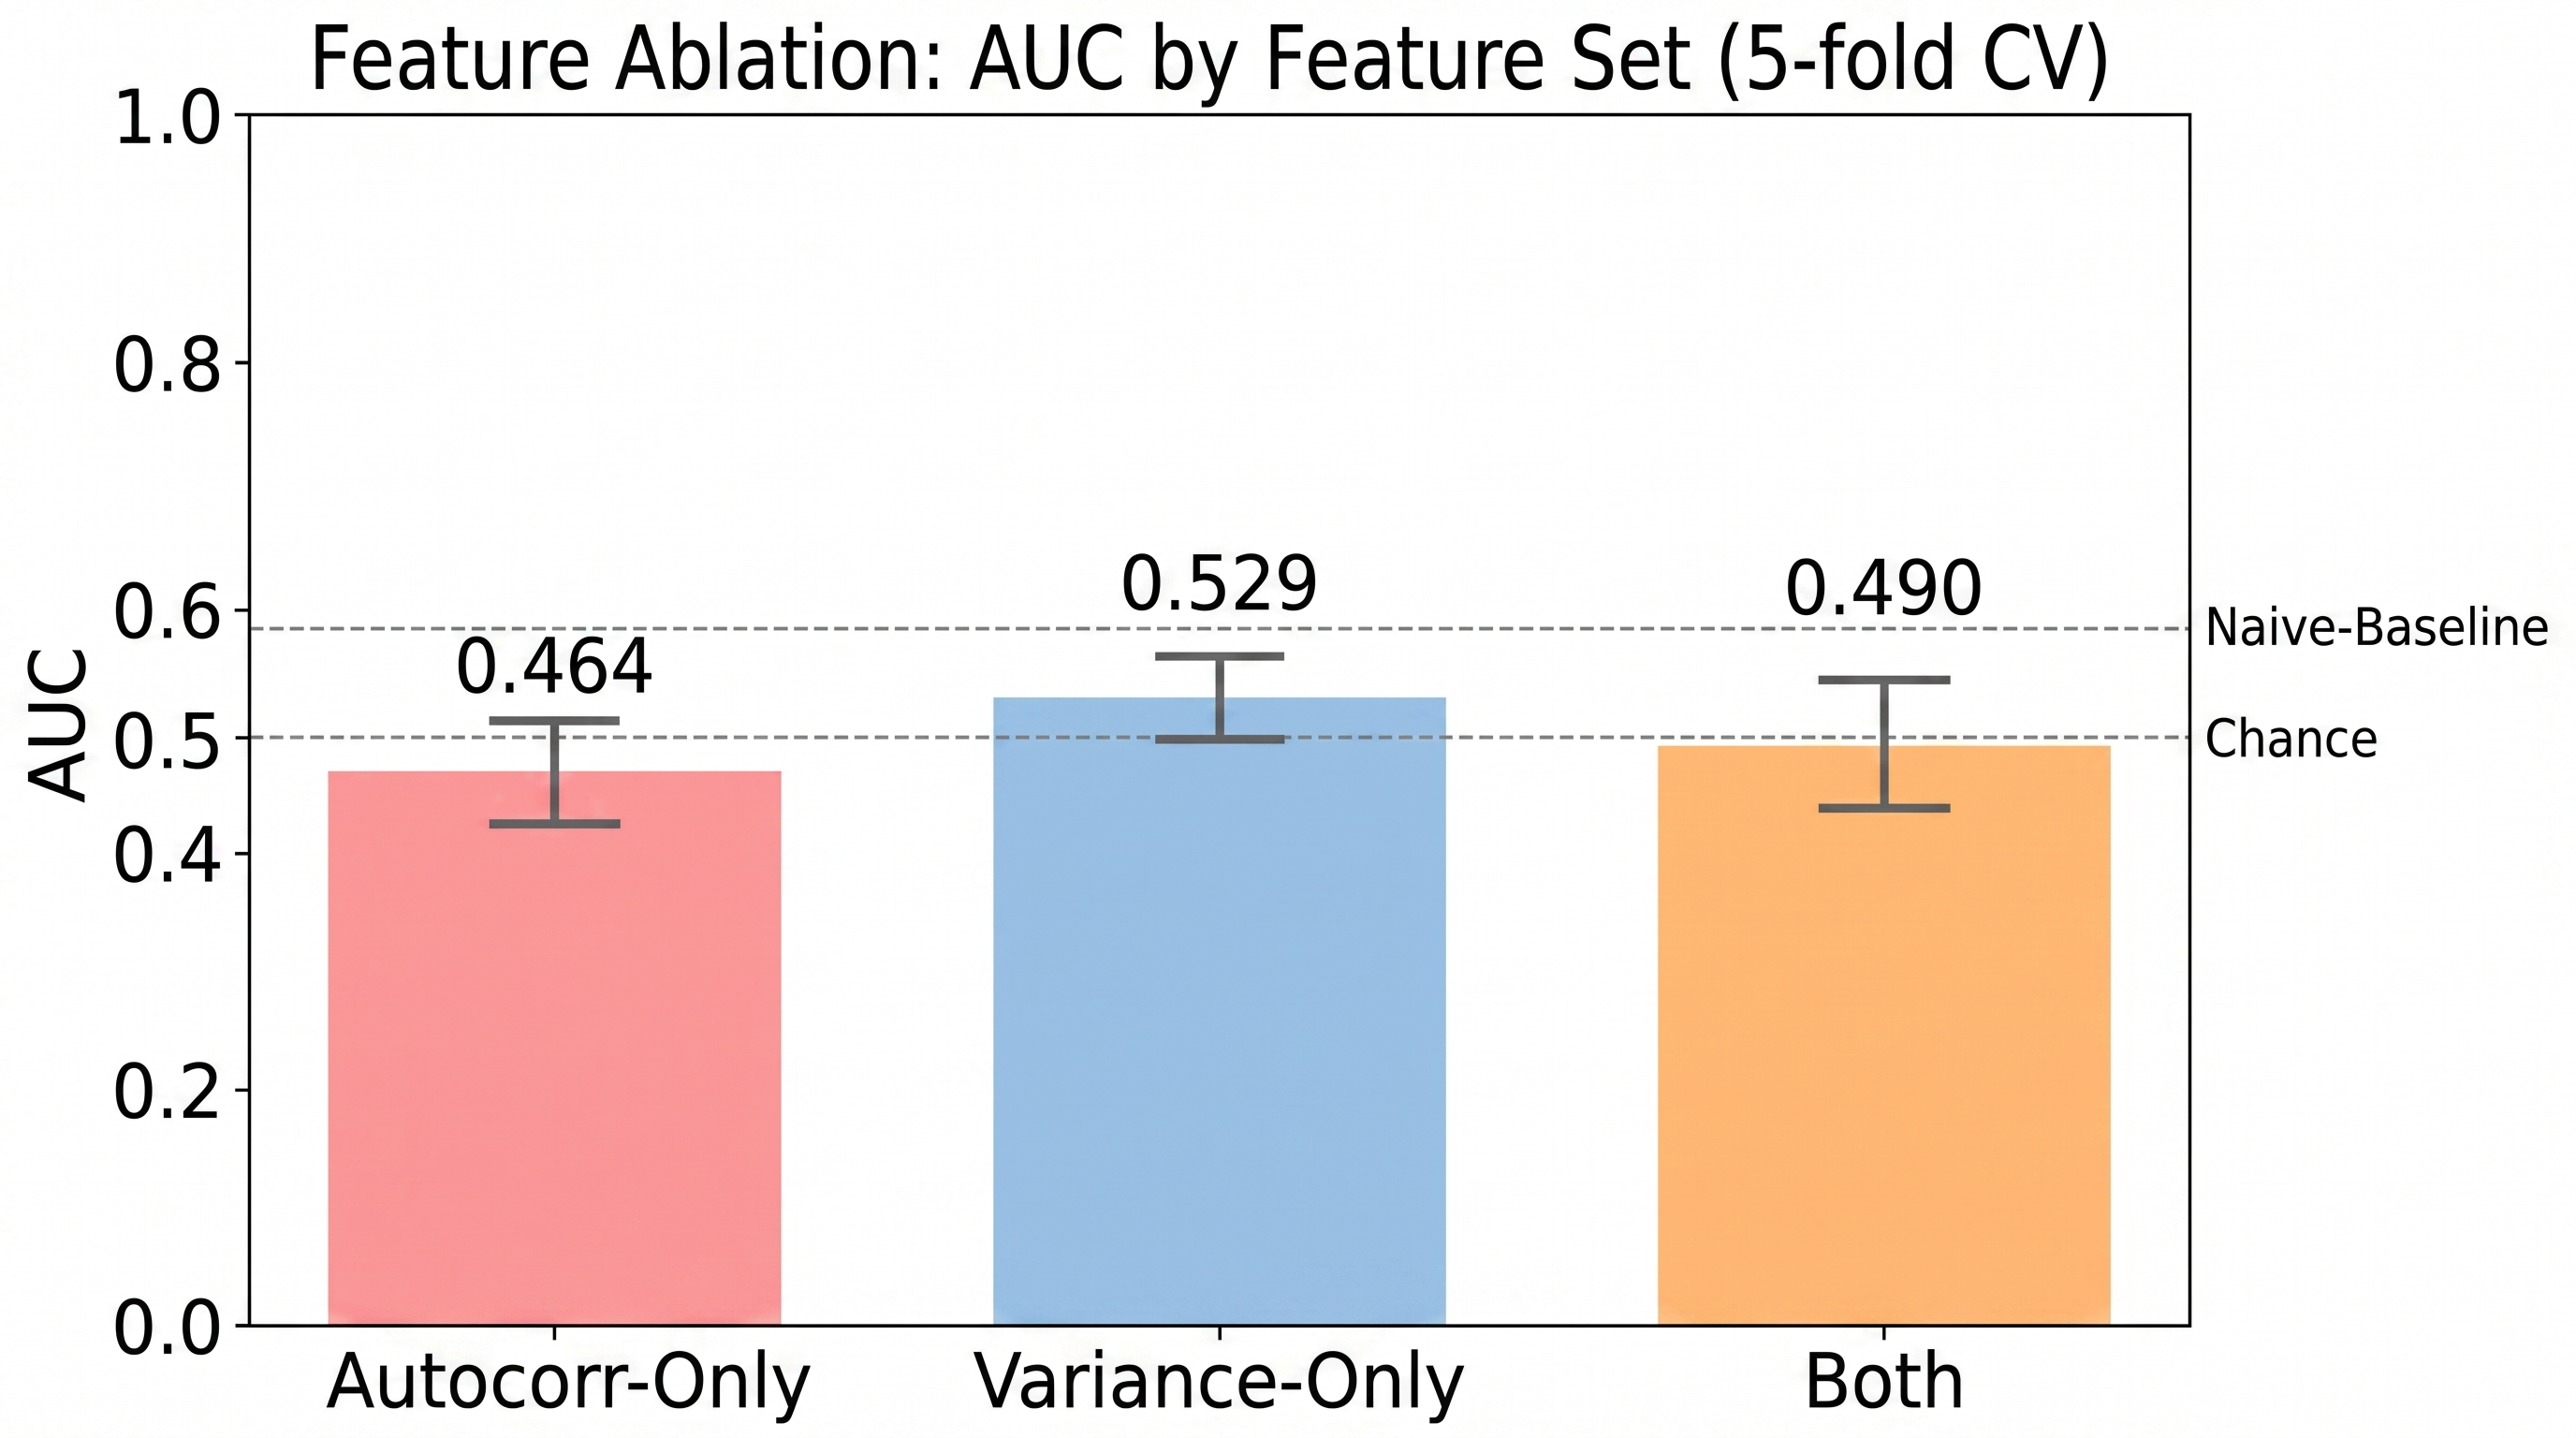
\includegraphics[width=\textwidth,height=0.45\textheight,keepaspectratio]{figures/fig3_v0.jpg}
  \caption{AUC when using autocorrelation alone, variance alone, or both features combined. Autocorrelation alone (AUC=0.464) performs below chance, variance alone (AUC=0.529) below baselines, and combined (AUC=0.490) is worse than variance alone, suggesting feature interactions are unhelpful or negatively correlated.}
  \label{fig:fig3}
\end{figure*}

When evaluated separately, autocorrelation-only achieves AUC = 0.464 (worse than chance), while variance-only achieves AUC = 0.529 (still below the naive baseline of 0.586). Combined, both features together degrade to AUC = 0.490, suggesting they provide negative information or are highly correlated with noise. Results are shown in Figure~\ref{fig:fig3}.

\subsection{Sensitivity Analysis: Robustness to Label Noise}

Excluding the memory\_simple\_voting config (which carries $\sim$24\% label mismatch):

\begin{table}[!htbp]
\centering
\caption{Sensitivity of AUC to exclusion of the noisy memory\_simple\_voting configuration.}
\label{tab:sensitivity}
\begin{tabular}{lccc}
\toprule
Classifier & Full AUC & Clean AUC & $|\Delta$ AUC$|$ \\
\midrule
CSD & 0.500 & 0.500 & 0.000 \\
Naive & 0.557 & 0.600 & 0.043 \\
Spectral & 0.576 & 0.167 & 0.409 \\
SPRT & 0.590 & 0.667 & 0.077 \\
\bottomrule
\end{tabular}
\end{table}

Results are not robust. The spectral model's AUC drops 40.9 percentage points when excluding the noisy config, indicating severe overfitting to label artifacts. CSD remains at chance (0.50) in both conditions.

\subsection{Lead-Time Analysis: No Advance Warning}

Lead time = rounds of advance warning before the debate's final round where the classifier fires an alarm. All debates in the dataset have exactly 7 rounds; alarm is measured relative to round 7. Results are shown in Table~\ref{tab:leadtime}.

\begin{table}[!htbp]
\centering
\caption{Mean lead time (rounds of advance warning) by classifier.}
\label{tab:leadtime}
\begin{tabular}{lcc}
\toprule
Classifier & Mean Lead Time (rounds) & SD \\
\midrule
CSD & 7.0 & 0.0 \\
Naive-agreement & 7.0 & 0.0 \\
Spectral & 7.0 & 0.0 \\
SPRT & 7.0 & 0.0 \\
\bottomrule
\end{tabular}
\end{table}

All classifiers fire at or after the debate concludes---no method provides actionable advance warning. This is because debates are uniformly short (exactly 7 rounds) and agreement converges quickly (by round 3--4, agreement is already $>$0.8). By the time any signal would fire, the debate is already effectively concluded.

\subsection{Colored-Noise Analysis and CSD Mechanism Absence}

We examined the power spectral density (PSD) of agreement trajectories to assess whether they exhibit colored noise (autocorrelated forcing) that might masquerade as CSD. Results:

\begin{itemize}
\item \textbf{Collapsed debates:} 68\% ``flat/no variation'' regime, 24\% white noise, 8\% low-frequency-peak (system dynamics)
\item \textbf{Converged debates:} 84\% ``flat/no variation'' regime, 13\% white noise, 2\% low-frequency-peak
\end{itemize}

The dominance of the ``flat'' regime (agreement constant or nearly constant across early rounds) explains the high NaN rate in autocorrelation and the absence of meaningful variance. There is no evidence of system oscillations or recovery dynamics that would manifest as CSD.

\section{Discussion}

\subsection{Why Critical Slowing Down Does Not Transfer to LLM Debates}

Our results provide clear evidence that the CSD hypothesis does not hold in multi-agent LLM debates. We identify several boundary conditions explaining this failure:

\textbf{1. No External Recovery Dynamics:} CSD in ecological systems arises from repeated, externally-driven perturbations (seasonal forcing, rainfall variability, human interventions) that push the system away from equilibrium and test its return rate. LLM debates lack this: there is no external perturbation during debate (unless a human or external verifier injects information, which does not occur in this corpus). Agreement dynamics are purely endogenous to agent updates. Without external recovery testing, slowing cannot manifest.

\textbf{2. Discretization and Saturation:} Agreement scores, computed as the fraction of agents sharing a modal solution, are discrete (e.g., 1/3, 2/3, 3/3 for 3 agents). Early rounds frequently exhibit agreement = 1.0 (full consensus) from the start, making the trajectory constant and autocorrelation undefined. In contrast, ecological systems measure continuous variables (e.g., lake nutrient concentration, forest biomass). Discretization leads to frequent saturation (agreement at ceiling) and high NaN rates for autocorrelation.

\textbf{3. Extremely Short Trajectories:} Debates consist of 3--7 rounds. Classical CSD methodology (per ecology literature) operates on time series of dozens to hundreds of observations per system. Rolling windows of size 2--3 on a 7-point series are at the extreme lower limit of statistical reliability. Permutation tests and bootstrap confidence intervals partially mitigate this, but cannot overcome the fundamental information scarcity.

\textbf{4. Bistability Unconfirmed:} CSD theory predicts bistability (competing attractor basins) as necessary. While MAST documents distinct failure outcomes, we have not explicitly measured bistability via state-space reconstruction or perturbation experiments. Debates may not exhibit true bistability---instead, agreement might be a unidirectional process (monolithic convergence once one position dominates) rather than a system poised between two competing basins.

\subsection{Why Simple Agreement Thresholds Succeed Where CSD Fails}

The naive agreement-score baseline (AUC = 0.586) outperforms CSD (AUC = 0.490). This suggests that the signal predictive of collapse is simply \emph{low agreement in early rounds}, not \emph{dynamics of agreement}. Conversations collapsing occur when agents remain distributed across multiple positions even after several rounds---a different phenomenon than low variance or slow recovery.

Intuitively, if after round 1 or 2 the agents have not converged to a single modal answer, the debate is less likely to converge \emph{correctly} by the final round. This is a simpler and more direct signal than reconstructing dynamical slowing. The spectral cascade model (AUC = 0.587) also outperforms CSD by similarly leveraging agent interaction structure, but is more complex to implement (requires citation graph inference).

\subsection{Methodological Contributions: How to Evaluate EWS on Short Time Series}

While the CSD hypothesis fails, this work makes a methodological contribution by establishing the proper approach for evaluating early-warning hypotheses on short, discrete time series:

\begin{enumerate}
\item \textbf{Permutation Testing:} Block-shuffled permutation tests (not parametric significance) are essential when rolling-window estimates are biased and unreliable (as they are for 2--3 point windows).

\item \textbf{Cross-Validation:} Train/test splits at the debate level (not round level) ensure no information leakage and test generalization to unseen debates.

\item \textbf{Robustness to Label Noise:} Sensitivity analysis excluding high-noise data sources is essential---spectral models' AUC collapsed 40 points when excluding noisy configs, indicating no robust signal.

\item \textbf{Feature Ablation:} Showing that autocorrelation-only performs worse than variance-only highlights that individual CSD components are uninformative.

\item \textbf{Lead-Time Measurement:} Computing when classifiers fire relative to debate termination clarifies whether signals are truly advance warnings or post-hoc observations. Our result (all methods fire at debate end) reveals that 7-round debates are too short for advance warning regardless of signal type.
\end{enumerate}

\subsection{Implications for Multi-Agent System Design}

This negative result has positive implications for practitioners:

\begin{enumerate}
\item \textbf{Simplicity is Better:} If the goal is early detection of problematic debates, simple agreement-score tracking suffices. No need for complex dynamics-based models.

\item \textbf{Extend Debate Duration:} For early warning to be actionable, debates must extend longer than 3--7 rounds. Current debate systems in the corpus terminate at round 7 by design, leaving no time to intervene after an early-warning signal fires. Extended debates (10--20 rounds) combined with simple agreement thresholds might enable mid-trajectory intervention.

\item \textbf{Focus on Intervention Mechanics, Not Detection:} Rather than perfecting early-warning prediction, focus on how to \emph{act} on such signals (how to diversify models, inject corrective information, halt debate gracefully without wasting prior rounds).
\end{enumerate}

\subsection{Limitations}

\begin{enumerate}
\item \textbf{Single Model Family:} The DEBATE corpus uses only Llama-3.3-70B agents with persona variation. Multi-model deployments (GPT-4, Claude, Llama, different sizes) may exhibit different agreement dynamics and cascade coefficients 3--5$\times$ larger or smaller \citep{Liu2026}.

\item \textbf{Single Task Domain:} Debates are yes/no factual questions. Mathematical reasoning (MATH), logical puzzles, or open-ended generation may show different convergence patterns.

\item \textbf{No Explicit Bistability Confirmation:} We assume debate dynamics exhibit bistability but have not measured it via perturbation experiments or state-space reconstruction.

\item \textbf{Lead-Time Ceiling:} All debates are exactly 7 rounds by design. True lead-time comparison requires longer sequences where advance warning can precede termination.
\end{enumerate}

\section{Conclusion}

We tested the hypothesis that critical slowing down---a generic early-warning signature from ecology---transfers to LLM multi-agent debate collapse. Using a real dataset of 95 authentic debates and rigorous cross-validation methodology, we find the hypothesis is \textbf{not supported}. CSD statistics (autocorrelation and rolling variance) perform at chance level (AUC = 0.490) and are substantially outperformed by naive agreement-score thresholds (AUC = 0.586) and spectral models (AUC = 0.587).

This negative result is scientifically valuable, contributing (1) a methodological framework for evaluating early-warning hypotheses on short, discrete time series via permutation testing and cross-validation, (2) evidence that simple agreement-level features already capture collapse-predictive information, and (3) identification of boundary conditions explaining CSD transfer failure: discretization of agreement, extremely short trajectories (3--7 rounds), absence of external recovery dynamics, and unconfirmed bistability.

Future work should investigate whether explicit perturbation experiments (injecting false/correct statements mid-debate and measuring recovery rate) reveal latent CSD signatures invisible in unperturbed trajectories, test generalization across longer debates and multi-model configurations, and develop intervention mechanics (how to act on early-warning signals when they do fire).

\subsection{Future Work}

\begin{itemize}
\item \textbf{Perturbation Experiments:} Inject false statements mid-debate; measure recovery rate as a direct test of critical slowing. Slower recovery in pre-collapse debates would validate the underlying mechanism.
\item \textbf{Extended Debate Trajectories:} Design debates to run 15--30 rounds, enabling true lead-time measurement and mid-trajectory interventions.
\item \textbf{Multi-Model and Multi-Task Evaluation:} Test generalization across GPT-4/Claude/Llama mixes and benchmarks (MATH, GSM8K, reasoning).
\item \textbf{Explicit Bistability Tests:} Reconstruct state-space attractor geometry via embedding; measure separatrix distance as an early warning for eventual basin boundary crossing.
\end{itemize}

\bibliographystyle{plainnat}
\bibliography{references}

\end{document}
